\documentclass[hperref={pdfpagelabels=false}]{beamer}

\usefonttheme[onlymath]{serif}
\usepackage{lmodern}
\usepackage[T1]{fontenc}
\usepackage[utf8]{inputenc}
\usepackage{hyperref}
\usetheme{default}
\usepackage{physics}
\usepackage{caption}
% \captionsetup{font=scriptsize,labelfont=scriptsize}
\usepackage{booktabs}

\usepackage{siunitx}
\DeclareSIUnit\solarmass{M_{\odot}}

\begin{document}

\title
{Computing project: Neutron star}

\subtitle{Neutron star modelled as pure Fermi gas with nucleon interaction}

\author
{Luis Caceres Cueva \and Tomoi Goto}

\institute
{
    School of Phsyics and Astronomy\\
    The University of Manchester
}
\date
{May 8, 2019}

\begin{frame}
 \titlepage
\end{frame}

\begin{frame}
    \frametitle{Structure equations}
    \begin{itemize}
        \item From hydrostatics, we get the Newtonian structure equation: \[\dv{p}{r}=-\frac{GM\rho}{r^{2}}\]
        \item With general relativistic corrections, we get the TOV equation: \[\dv{p}{r}=-\frac{GM\rho}{r^{2}}\qty[1+\frac{p}{\epsilon}]\qty[1+\frac{4\pi r^{3}p}{Mc^{2}}]\qty[1-\frac{2GM}{c^{2}r}]^{-1}\]
        \item From definition of the mass of a spherical shell: \[\dv{M}{r}=4\pi r^{2}\rho\]
    \end{itemize}
\end{frame}

\begin{frame}
    \frametitle{Fermi gas model}
    \begin{itemize}
        \item We define the dimensionless quantity \[x\equiv\frac{\hbar k_{F}}{mc}\]
    \item Hence, we can write the relevant physical quantities
        \begin{align*}
            n&=n_{0}x^{3},&n_{0}&=\frac{m^{3}c^{3}}{3\pi^{2}\hbar^{3}},\\
            \rho&=\rho_{0}x^{3},&\rho_{0}&=\frac{m^{4}c^{3}}{3\pi^{2}\hbar^{3}},\\
            \epsilon&=\epsilon_{0}x^{3}I(x),&\epsilon_{0}&=\frac{m^{4}c^{5}}{3\pi^{2}\hbar^{3}},\\
            p&=\frac{1}{3}\epsilon_{0}x^{4}I'(x),
        \end{align*}
    where \[I(x)\equiv \frac{3}{8x^{3}}\qty[x(1+2x^{2})(1+x^{2})^{1/2}-\log(x+\sqrt{1+x^{2}})]\]
    \end{itemize}
\end{frame}


\begin{frame}
    \frametitle{Fermi gas model with nucleon interaction}
    \begin{itemize}
        \item We define the dimensionless quantity \[u\equiv\frac{n}{n_{S}}=\frac{x^{3}}{\eta}\] % where $n_{S}$ is the number density at saturation and $\eta=n_{S}/n_{0}$ is a ratio between constants.
        \item We parametrize the asymmetry between neutrons and protons with $\alpha$, such that \begin{align*}n_{p}&=\frac{1-\alpha}{2}n&n_{n}&=\frac{1+\alpha}{2}n\end{align*}
        \item Using the classical approximation for kinetic energy, the energy per particle is \[\frac{\epsilon}{n}=mc^{2}+E_{N}u^{2/3}+V(u)+\alpha^{2}S(n),\] where \[E_{N}=\frac{3}{10}mc^{2}\eta^{2/3}\]
    \end{itemize}
\end{frame}

\begin{frame}
    \frametitle{Fermi gas model with nucleon interaction}
    \begin{itemize}
        \item We use as the symmetry breaking potential: \[S(n)=E_{N}(2^{2/3}-1)\qty(u^{2/3}-F(u))+S_{0}F(u),\] where $F(u)$ is an arbitrary function such that $F(0)=0$ and $F(1)=1$.
        \item We use as the nucleon interaction potential: \[V(u)=\frac{A}{2}u+\frac{Bu^{\sigma}}{(1+\sigma)(1+C_{1}u^{\sigma-1})}\]
        \item The parameters of $V(u)$ are fitted to the properties of nuclear matter at saturation density:
            \begin{align*}
                \qty(\dv{u}\qty[\frac{\epsilon(n)}{n}])_{u=1}&=0,&\frac{\epsilon(n_{1})}{n_{1}}-mc^{2}&=E_{B},\\
                K(n_{1})=9\dv{p}{n}&=K_{0},&\qty(\frac{c_{s}}{c})^{2}=\dv{p}{\epsilon}&<1
            \end{align*}
    \end{itemize}
\end{frame}

\begin{frame}
    \frametitle{Fermi gas model with nucleon interaction}
    \begin{itemize}
        \item Choosing \[F(u)=\sqrt{u},\] we can write the pressure for pure neutron matter ($\alpha=1$): \[p=E_{N}n_{1}J(u),\] where \[\resizebox{.8\textwidth}{!}{$\displaystyle J(u)\equiv u^{2}\qty[\frac{2}{3}u^{-1/3}+\frac{V'(u)}{E_{N}}+(2^{2/3}-1)\qty(\frac{2}{3}u^{-1/3}-F'(u))+\frac{S_{0}}{E_{N}}F'(u)]$}.\]
        \item We also choose $C_{1}=0.3$ as in Prakash, Aisnworth and Lattimer (1988) and we considered different values of $K_{0}$ between \SI{100}{\mega\electronvolt} and \SI{400}{\mega\electronvolt}.
    \end{itemize}
\end{frame}

\begin{frame}
    \frametitle{TOV equation in terms of density}
    \begin{itemize}
        \item Given the difficulty of explicitly writing $\rho$ in terms of $p$, we instead write the TOV equation in terms of $\rho$: \[\dv{\rho}{r}=-\qty(\dv{p}{\rho})^{-1}\frac{G\rho M}{r^{2}}\qty[1+\frac{p}{\epsilon}]\qty[1+\frac{4\pi r^{3}p}{Mc^{2}}]\qty[1-\frac{2GM}{c^{2}r}]^{-1}\]
        \item The derivative $\dv{p}{\rho}$ can be calculated relatively easily by applying the chain rule with respect to $x$.
    \end{itemize}
\end{frame}

\begin{frame}
    \frametitle{Dimensionless equations for Fermi gas model}
    \begin{itemize}
        \item To minimize floating point errors, we use dimensionless quantities:
            \begin{align*}
                \bar{r}&=\frac{r}{r_{0}},&\bar{M}&=\frac{M}{M_{0}},\\
                \bar{\rho}&=\frac{\rho}{\rho_{0}},&\bar{p}&=\frac{p}{\epsilon_{0}},\\
                \bar{\epsilon}&=\frac{\epsilon}{\epsilon_{0}}.
            \end{align*}
        \item Similarly, the equations have to be written in terms of the dimensionless quantities:
            \begin{align*}
                \dv{\bar{\rho}}{\bar{r}}&=-\qty(\frac{GM_{0}}{c^{2}r_{0}})\qty(\dv{\bar{p}}{\bar{\rho}})^{-1}\frac{\bar{M}\bar{\rho}}{\bar{r}^{2}}\qty[1+\frac{\bar{p}}{\bar{\epsilon}}]\qty[1+\frac{\bar{r}^{3}\bar{p}}{\bar{M}}]\qty[1-\frac{2\bar{M}}{\bar{r}}]^{-1}\\
                \dv{\bar{M}}{\bar{r}}&=\qty(\frac{4\pi r_{0}^{3}\rho_{0}}{M_{0}})\bar{\rho}\bar{r}^{2}
            \end{align*}
            where $M_{0}$ and $r_{0}$ are chosen such that the coefficients are equal to unity.
    \end{itemize}
\end{frame}

\begin{frame}
    \frametitle{Estimating the error of RK4 method}
    \begin{itemize}
     \item The main source of error is truncation error.
    \end{itemize}
    \begin{itemize}
     \item It can be estimated by integrating at two different step sizes $h_{1}=2h$ and $h_{2}=h$, which result in $Y_{1}$ and $Y_{2}$
    \end{itemize}
    \begin{itemize}
     \item From these, the error on $Y_{2}$ at step size $h_{2}=h$ is \[E_{2}=(Y_{1}-Y_{2})/15.\]
    \end{itemize}
\end{frame}

\begin{frame}
    \frametitle{Maximum masses and radii}
    \begin{table}[h]\begin{center}
        \caption{Maximum masses and radii at maximum mass of neutron stars for a given nuclear incompressibility $K_0$}
        \begin{tabular}{ccc}
            \toprule
            $K_{0}$ (\si{\mega\electronvolt}) & $M_{\text{max}}$ (\si{\solarmass}) & $R_{\text{max}}$ (\si{\kilo\meter}) \\
            \midrule
            \num{100} & \num{1.36} & \num{6.78}\\
            \num{175} & \num{2.01} & \num{8.30}\\
            \num{250} & \num{2.30} & \num{9.25}\\
            \num{325} & \num{2.27} & \num{9.68}\\
            \num{400} & \num{1.97} & \num{9.80}\\
            \bottomrule
        \end{tabular}
    \end{center}\end{table}
\end{frame}


\begin{frame}
 \frametitle{Comparison between our models}
 \begin{figure}
    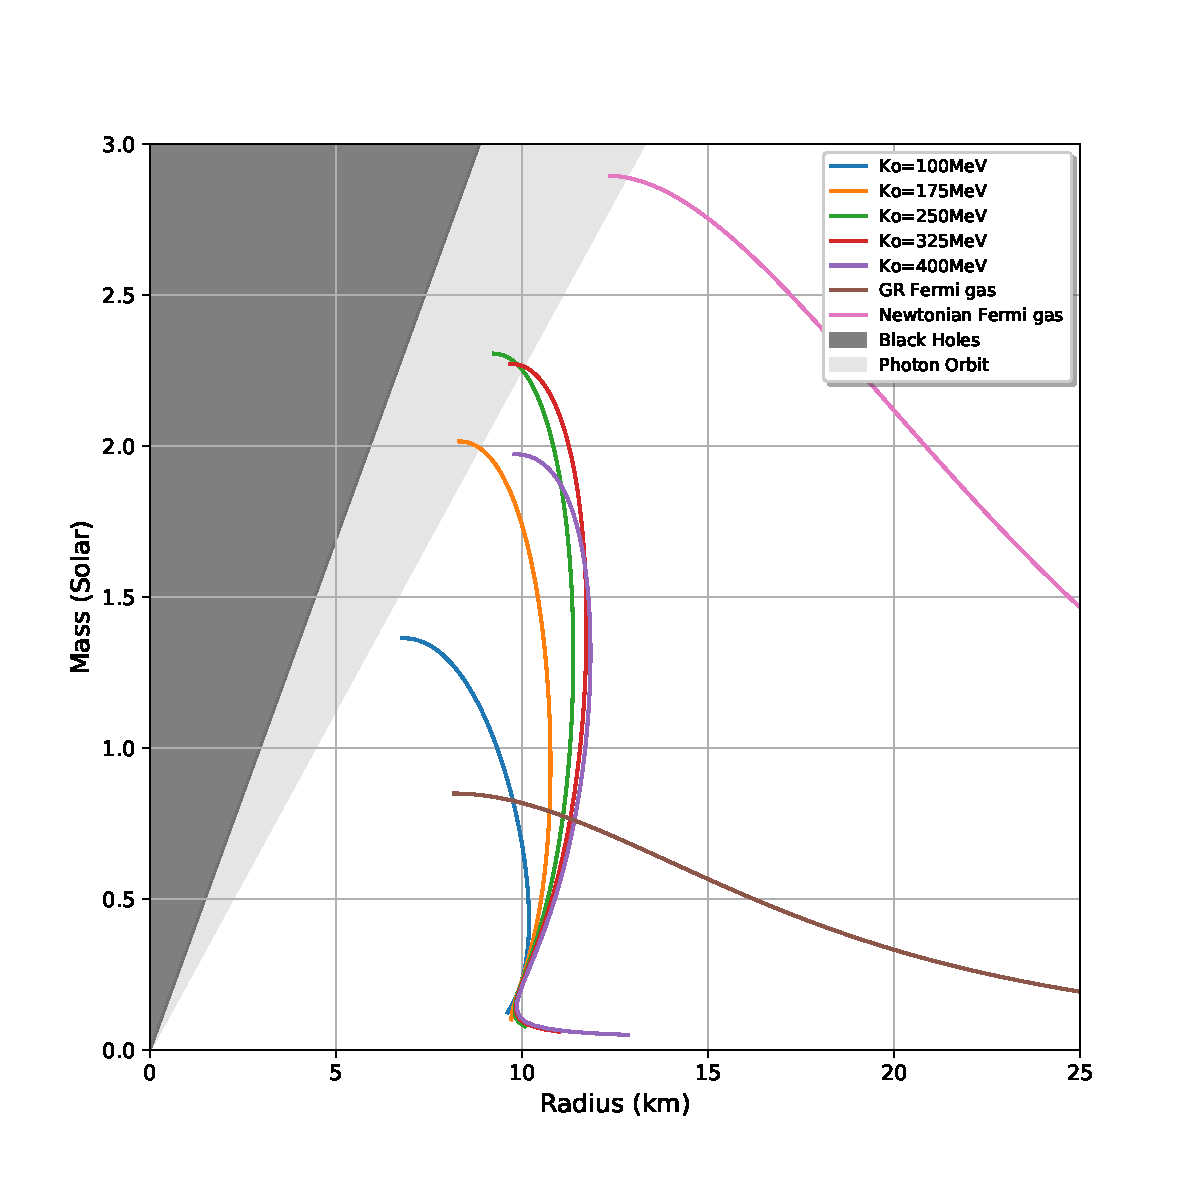
\includegraphics[scale=0.3]{eos_compare_our_model.pdf}
    \caption{Comparison between Fermi gas with Newtonian structure, General Relativistic structure, and model with nucleon interactions of different stiffness ($K_{0}$).}\label{fig/ourmodel}
  \end{figure}
\end{frame}

\begin{frame}
 \frametitle{Comparison with models from the literature}
 \begin{figure}
    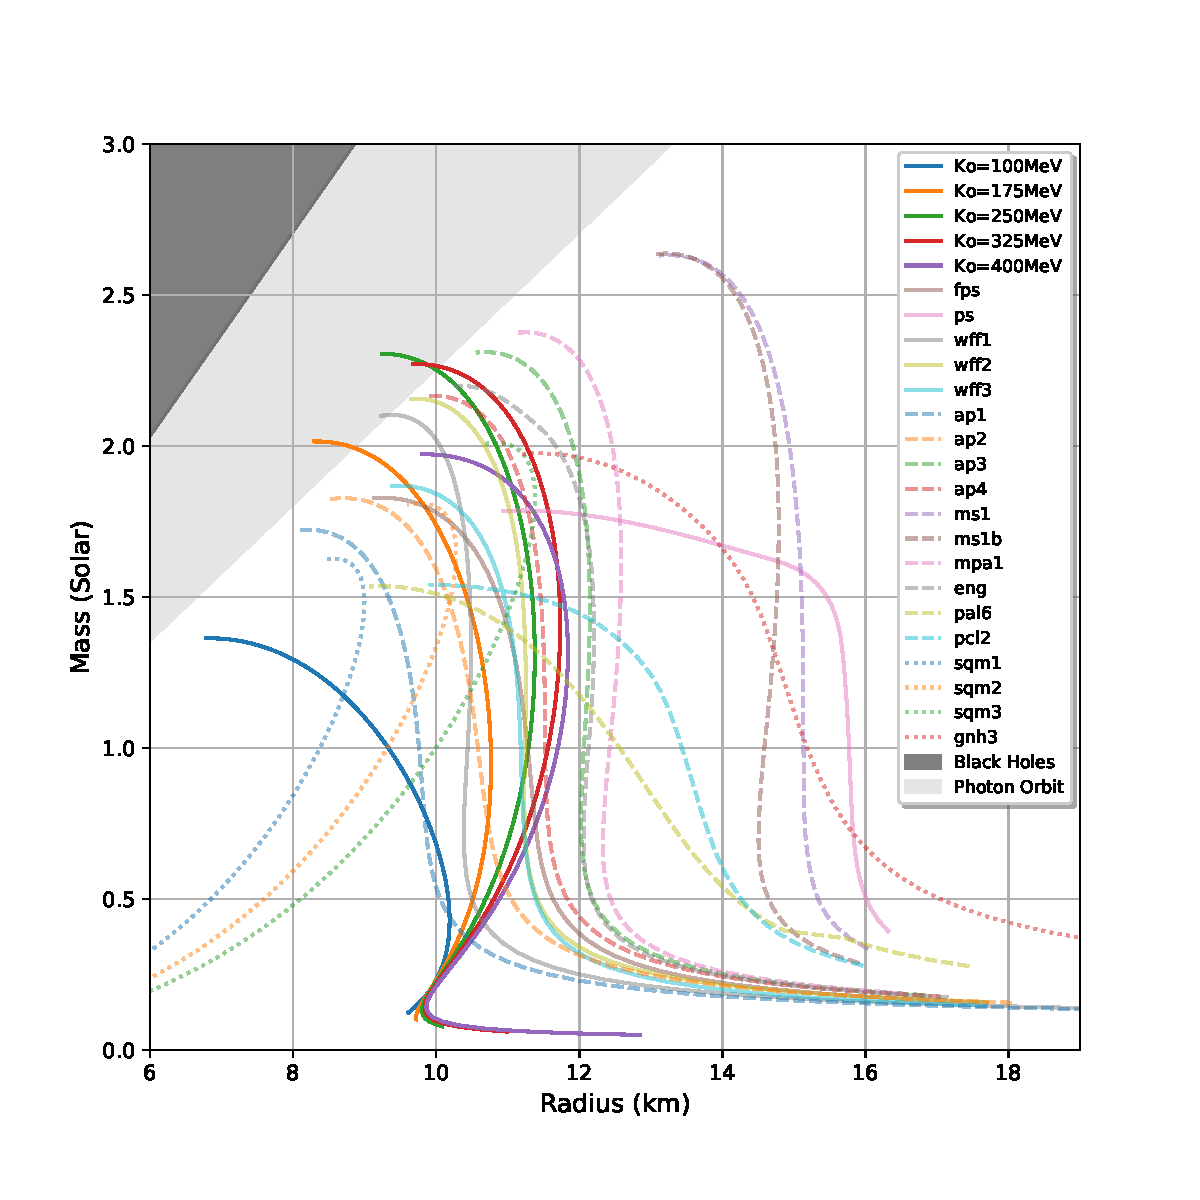
\includegraphics[scale=0.3]{eos_compare_paper.pdf}
    \caption{Comparison between Fermi gas model with nucleon interactions to other EOS models in the literature.}
 \end{figure}
\end{frame}

\begin{frame}
 \frametitle{Comparison with observation data}
 \begin{figure}
    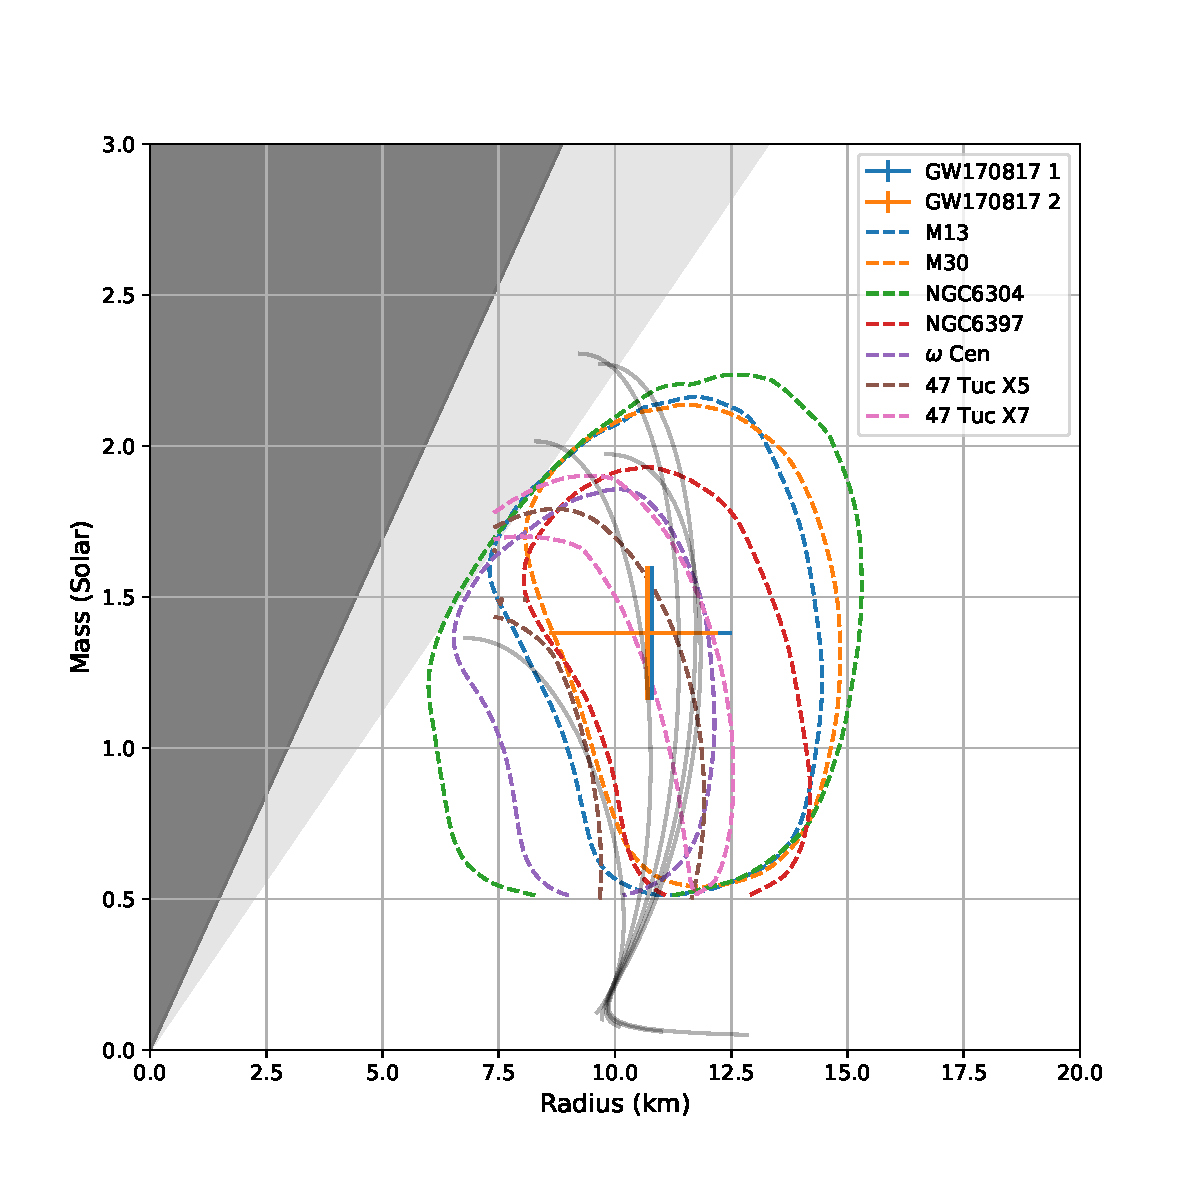
\includegraphics[scale=0.3]{eos_compare_obsv1_GW.pdf}
    \caption{Comparison between our models with observations from quiescent low mass X-ray binaries and gravitational wave event.}
 \end{figure}
\end{frame}

\begin{frame}
 \frametitle{Comparison with observation data}
 \begin{figure}
    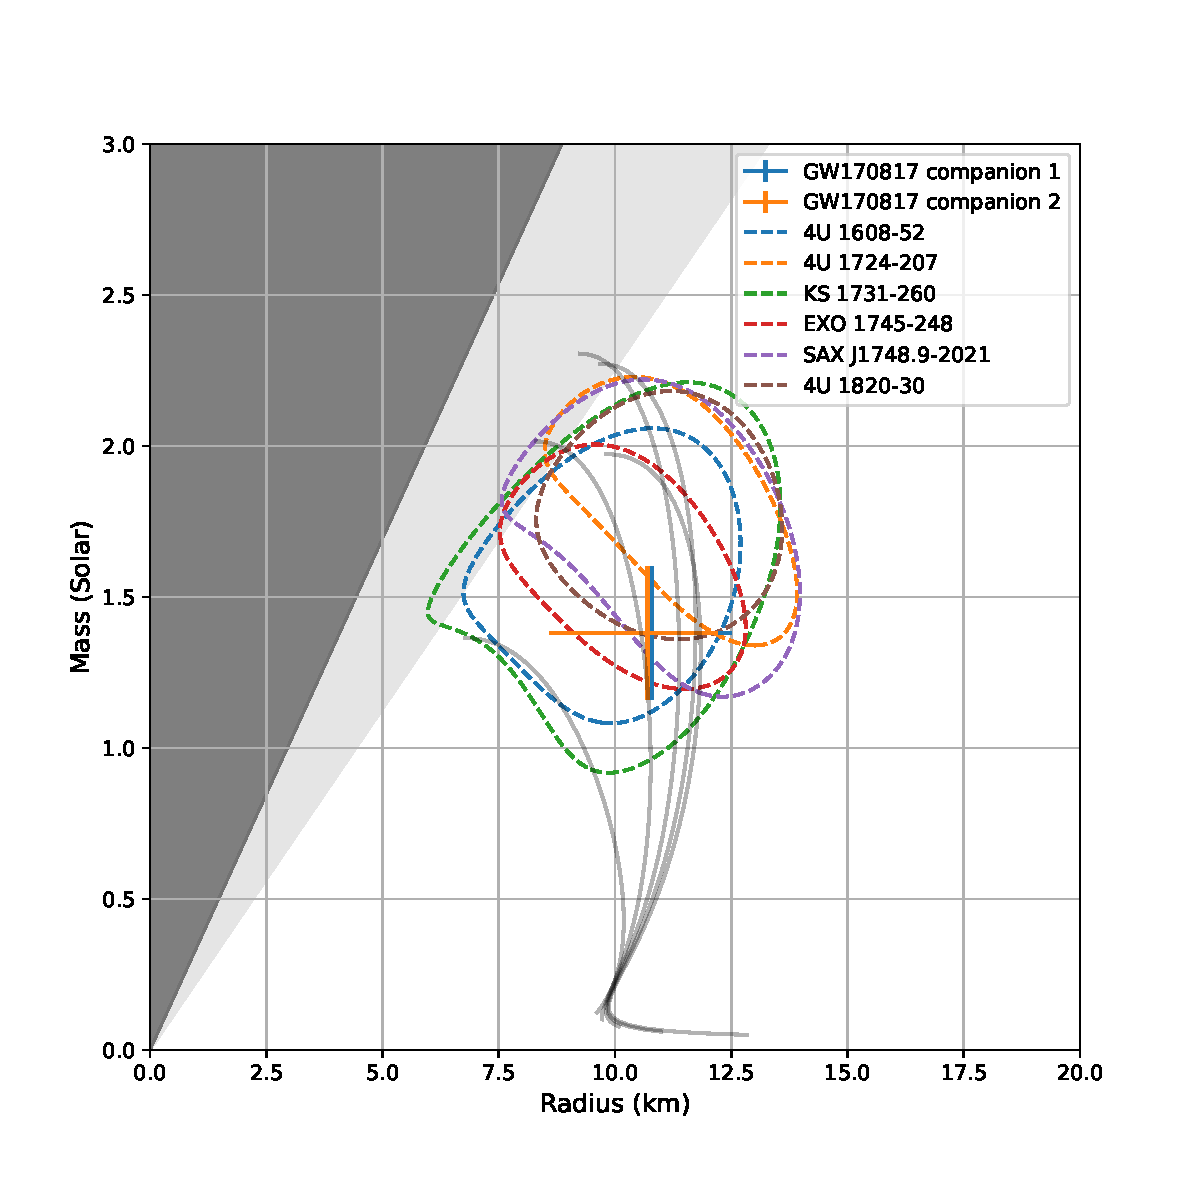
\includegraphics[scale=0.3]{eos_compare_obsv2_GW.pdf}
    \caption{Comparison between our models with observations from thermonuclear bursts of LMXBs and gravitational wave event.}
 \end{figure}
\end{frame}

\end{document}
